% $Id$

\chapter{Block design fMRI dataset}
\label{sec:Block_design_fMRI_dataset}
\minitoc

This chapter will describe the steps necessary to perform a classification using PRoNTo. The dataset\footnote{Pre-processed (realigned and normalised) data from participant 1.} used in this chapter can be found in PRoNTo's website \url{http://www.mlnl.cs.ucl.ac.uk/pronto/prtdata.html} (data set 1) and the whole\footnote{Not pre-processed.} dataset is available in \url{http://data.pymvpa.org/datasets/haxby2001/}.

This fMRI dataset originates from a study on face and object representation in human ventral temporal cortex \cite{Haxby2001}. In this study, the subject was shown a set of grey scale images of 8 categories (faces, houses, cats, chairs, bottles, scissors, shoes and scrambled pictures), with 12 runs/blocks. Each image was displayed for 500 ms and was followed by a 1500 ms rest interval. This experiment consisted on a block-design of 9 scans of task followed by 6 scans of inter-stimulus interval. Images were acquired with a TR of 2.5 s. The full-brain fMRI data was made up by 1452 volumes with 40 x 64 x 64 voxels, each of which with dimensions of 3.5 x 3.75 x 3.75 mm.

For simplicity, in this example we will use PRoNTo to predict if the subject is viewing an image of a Face or a House based on the fMRI scans. We will classify the whole brain images using Support Vector Machines, and a leave one block out cross-validation scheme.

\section{GUI analysis}

We will first analyse the data using PRoNTo's GUI and then repeat the analysis using the {\tt matlabbatch} system.

To start, create a new directory in which to save the results of the analysis, then start up MATLAB and type `prt' or `pronto' in the MATLAB prompt. This will open the main interface of PRoNTo (Figure \ref{fig:mainInterface}).

\begin{figure}[!h]
	\centering
		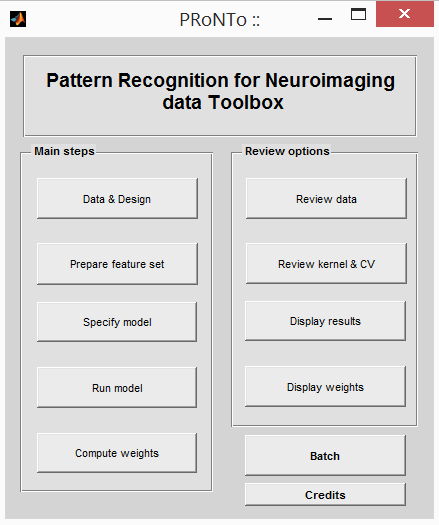
\includegraphics[scale=0.8]{images/Tutorial/classification/mainInterface.png}
	\caption{Main interface of PRoNTo.}
	\label{fig:mainInterface}
\end{figure}

%--------------------------------------------------------------------------
\subsection{Data \& Design}

\begin{itemize}
	
	\item In PRoNTo's main window, click on `Data \& Design' and a new window will open, `Data and design' (Figure \ref{fig:dataDesign}). Then, browse the directory in which to save the PRT structure (saved as `PRT.mat');
	
\begin{figure}[!h]
	\centering
			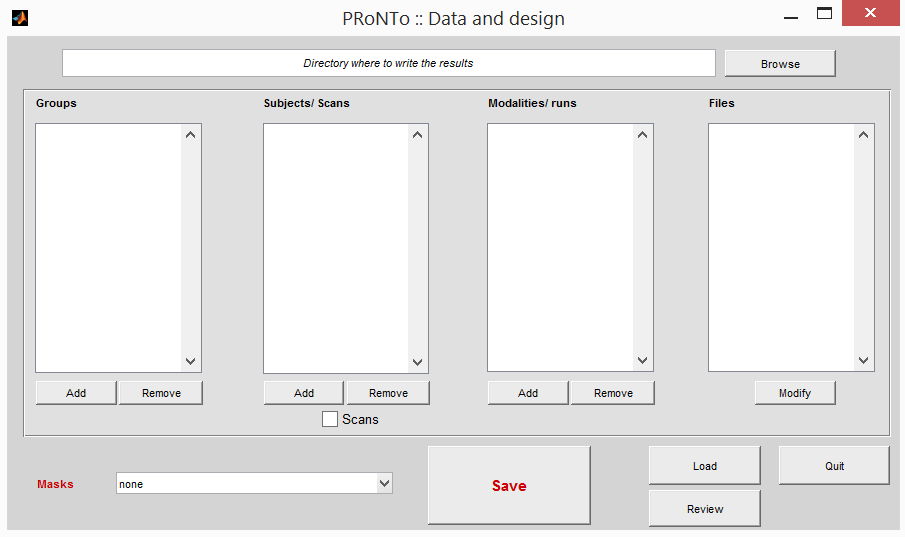
\includegraphics[scale=0.7]{images/Tutorial/classification/dataDesign.png}
	\caption{`Data and design' GUI.}
	\label{fig:dataDesign}
\end{figure}
	
	\item In the panel `Groups', click on `Add' and provide a name to the group (we only have one group/subject), with no spaces, e.g. `G1';
	
	\item Add a subject in the `Subject/Scans' option, e.g. `s1', and leave the `Scans' tick box below the panel unchecked. See Chapter \ref{chap:DataDesign} of the manual for more information on this option;
	
	\item In the `Modalities' panel, click on `Add' and provide a name to the modality, e.g. `fMRI'. In the `Design' field, choose the option `Load SPM.mat' (Figure \ref{fig:modality}). This file is available with the Haxby dataset on PRoNTo's website\footnote{http://www.mlnl.cs.ucl.ac.uk/pronto/prtdata.html} inside the folder Haxby\_dataset/design/;
	
\begin{figure}[!h]
	\centering
		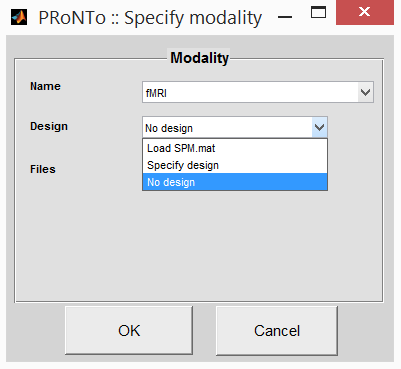
\includegraphics[scale=0.7]{images/Tutorial/classification/modality.png}
	\caption{`Specify modality' GUI allows one to load a specified design from an `SPM.mat' file.}
	\label{fig:modality}
\end{figure}

	\begin{itemize}
	
		\item In case there is no `SPM.mat' file available to use, create a new design by selecting the option `Specify design'. Choose how many conditions you have, which in this case are 8 conditions (corresponding to the 8 categories of images). This will open another window that allows the user to write the names, onsets and durations (if the duration is the same for all events only one value is required) of each condition (Figure \ref{fig:specifyDesign}). The unit in which the onsets/durations are read in this case is `scans' and the interscan interval (TR) is 2.5 seconds. The design information (names, onsets and durations) can be found inside the `Haxby\_design.pdf' file in the Haxby dataset folder. 
	
	\end{itemize}
	
\begin{figure}[!h]
	\centering
		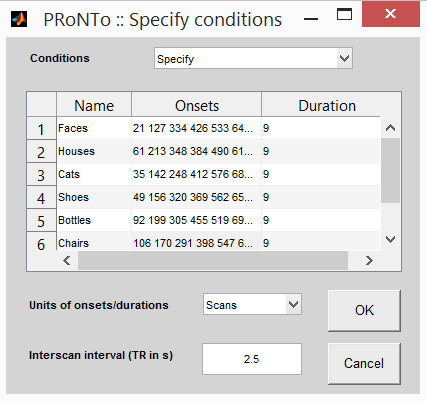
\includegraphics[scale=0.7]{images/Tutorial/classification/specifyDesign.png}
	\caption{`Specify design' GUI to enter the conditions, the units of design, TR and covariates.}
	\label{fig:specifyDesign}
\end{figure}
	
	\item Finally, load all the image files available in the fMRI directory (Haxby\_dataset/fMRI/). You can select all the files by using the right mouse button and clicking on the option `Select All' (Figure \ref{fig:files}). When all the images are selected, click on the `Done' button;
	
		
\begin{figure}[!h]
	\centering
		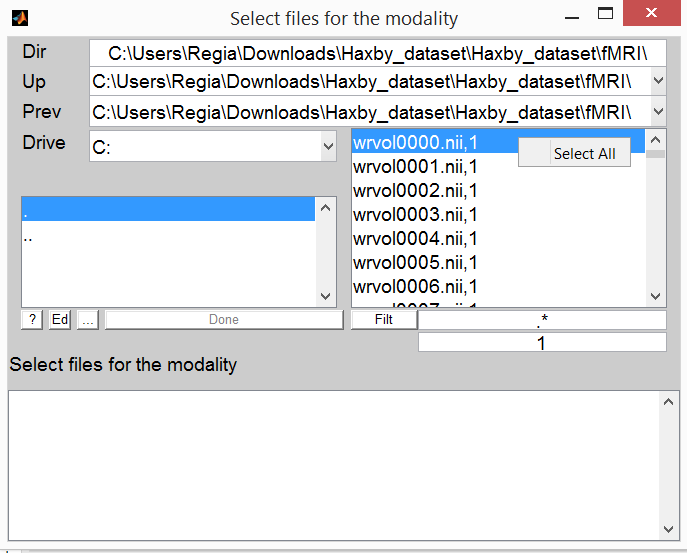
\includegraphics[scale=0.65]{images/Tutorial/classification/files.png}
	\caption{`Files' field is used to select the scans/images for the selected subject.}
	\label{fig:files}
\end{figure}
	
	\item In the `Masks' field, on the bottom left of the `Data and design' window, select the `whole\_brain' mask for the modality specified (Figure \ref{fig:mask}). The mask is available in the masks directory inside the folder Haxby\_dataset/masks/;

\begin{figure}[!h]
	\centering
		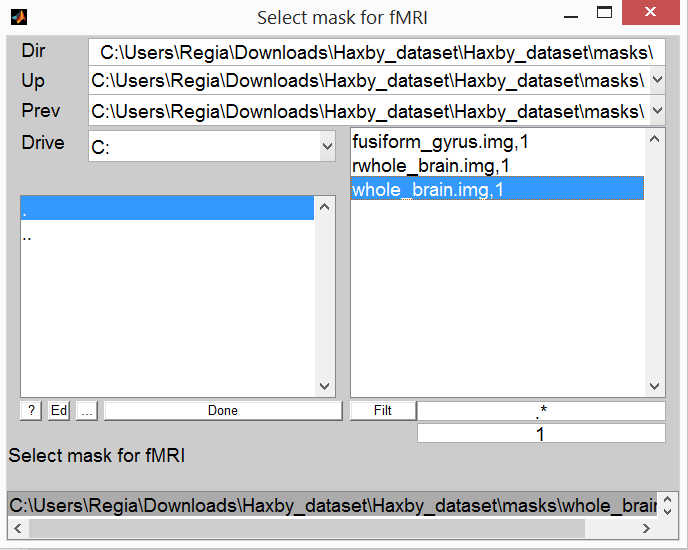
\includegraphics[scale=0.65]{images/Tutorial/classification/mask.png}
	\caption{This window is called when one clicks `Masks'.}
	\label{fig:mask}
\end{figure}

	\item Click on `Review' button to check the data and the design inserted in this modality (Figure \ref{fig:review}). For more information on what one can do with the Review option please see Chapter \ref{chap:DataDesign};
	
	
\begin{figure}[!h]
	\centering
		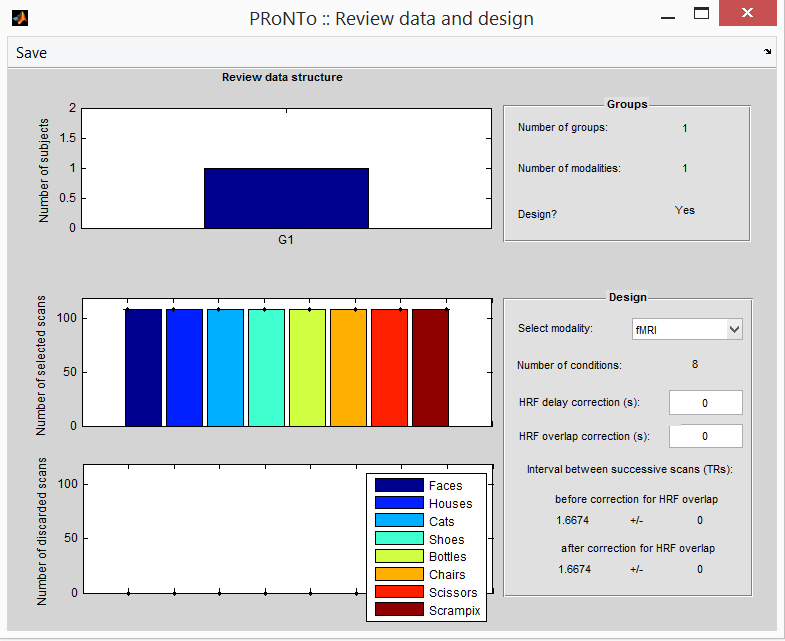
\includegraphics[scale=0.7]{images/Tutorial/classification/review.png}
	\caption{`Review' GUI allows the user to check the data and design.}
	\label{fig:review}
\end{figure}	
	
	\item The `Data and design' window should look similar to the Figure \ref{fig:finalDesign}. Click on `Save' button to create `PRT.mat' file with the structure containing the information that has been previously specified. If no errors are shown in the MATLAB command window, leave the `Data and design' window by clicking `Quit'.
	

\begin{figure}[!h]
	\centering
		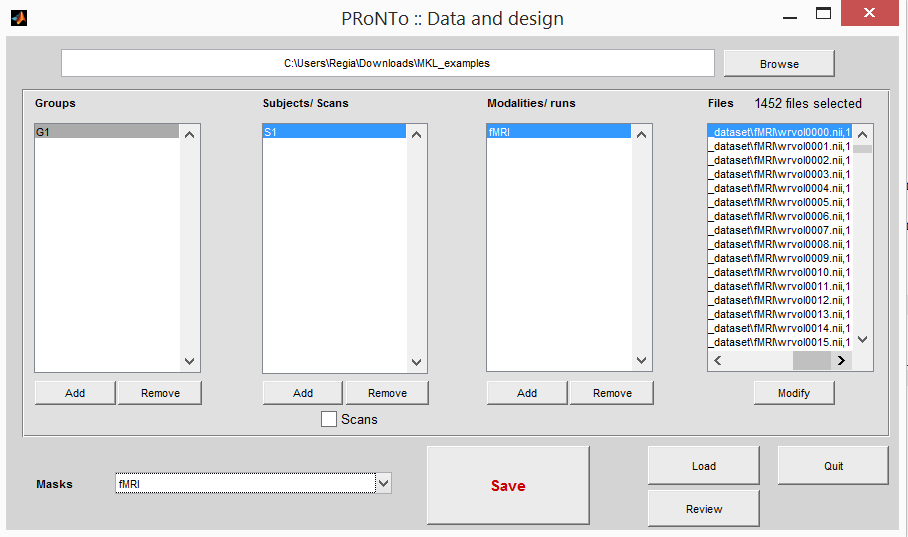
\includegraphics[scale=0.7]{images/Tutorial/classification/finalDesign.png}
	\caption{`Data and design' GUI final configuration.}
	\label{fig:finalDesign}
\end{figure}	

\end{itemize}

%--------------------------------------------------------

\subsection{Prepare feature set}

\begin{itemize}
	
	\item In PRoNTo's main window, click on `Prepare feature set' and a new window will open, `Prepare feature set' (Figure \ref{fig:prepareFeature});
	
	\begin{figure}[!h]
	\centering
		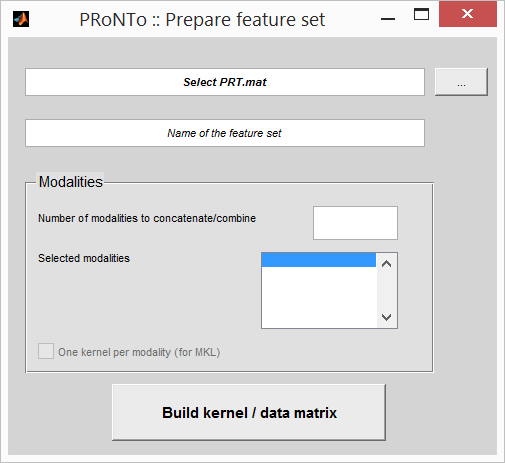
\includegraphics[scale=0.7]{images/Tutorial/classification/prepareFeature.png}
	\caption{`Prepare feature set' GUI.}
	\label{fig:prepareFeature}
\end{figure}
	
	\item Select the `PRT.mat' file previously created in the `Data \& Design' step and another window will open, `Specify modality to include' (Figure \ref{fig:specifyModality}), to set the specification of different parameters and options for each modality, which are: 
	
	\begin{itemize}
		\item `Modality' field: select the modality previously specified in the `Data \& Design' step, `fMRI';
		\item `Conditions' field: select `All scans'; 
		\item Parameters box: select the polynomial detrend with order 1 and the 'No scaling' option;
		\item Features box: leave the additional mask field as it is and the `build one kernel per region' tick box unchecked. Then, click on the `Done' button.  
		
			\begin{itemize}
			\item As an optional step, in the `Additional mask for selected modality' field, the user can specify a `second-level' mask, which can be used to select regions of interest (ROIs) on which the classification can be performed. For instance, we can enter the `fusiform\_gyrus' mask available with this dataset; 
			\end{itemize}	
			
			\begin{figure}[!h]
	\centering
		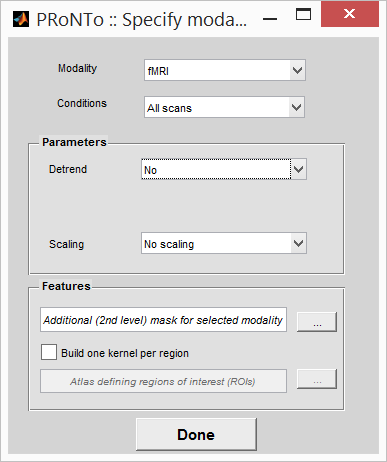
\includegraphics[scale=0.75]{images/Tutorial/classification/specifyModality.png}
	\caption{`Specify modality to include' GUI.}
	\label{fig:specifyModality}
\end{figure}				
		
	\end{itemize}		
		
	\item In the `Prepare feature set' window, provide a name for the feature set, e.g. `HaxbyFeatures';

	\item Click on `Build kernel/data matrix' to build the feature set and kernel (Figure \ref{fig:buildKernel}). It takes a few minutes.


\begin{figure}[!h]
	\centering
		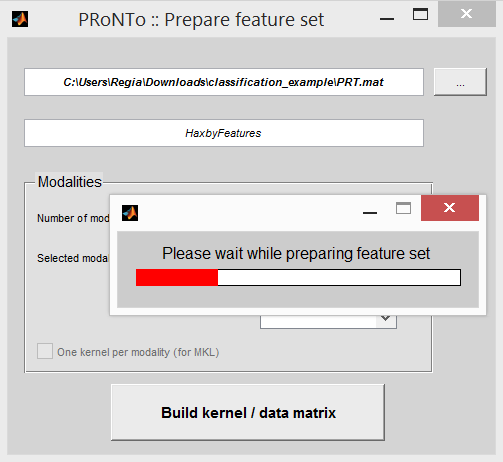
\includegraphics[scale=0.65]{images/Tutorial/classification/buildKernel.png}
	\caption{Preparing feature set.}
	\label{fig:buildKernel}
\end{figure}


\end{itemize}



%---------------------------------------------------------------------

\subsection{Specify model}

\begin{itemize}
	
	\item In PRoNTo's main window, click on `Specify model' and a new window will open, `Specify model' (Figure \ref{fig:specifyModel});
	
	\begin{figure}[!h]
	\centering
		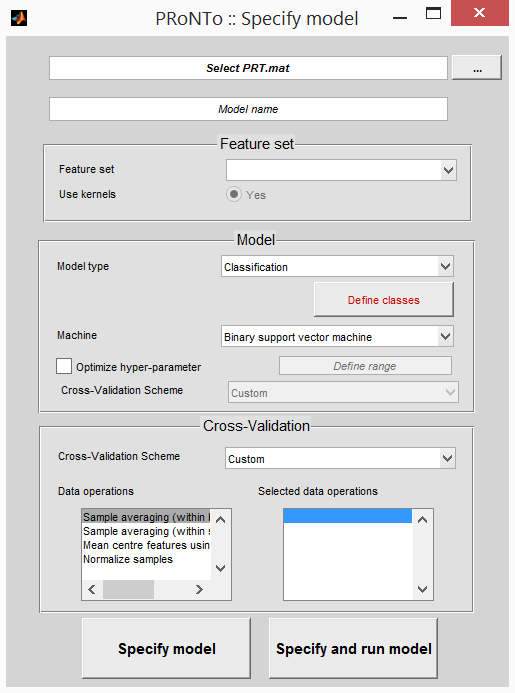
\includegraphics[scale=0.7]{images/Tutorial/classification/specifyModel.png}
	\caption{`Specify Model' GUI.}
	\label{fig:specifyModel}
\end{figure}
	
	\item Select the `PRT.mat' file and provide a name to the model, e.g. `svmFacesHouses';

	\item Select one of the `Feature Set' previously defined. In this case, there is only one `HaxbyFeatures';

	\item	Leave the option `Use kernels' tick box as it is, i.e. `Yes';

	\item	Select the `Classification' model type and click on `Define classes` button. A new window will open, `Specify classes' (Figure \ref{fig:specifyClasses}), to define the number of classes and a name for each class. We will define 2 classes. For `Class 1' select subject `S1' and the condition `Faces' and, similarly, for `Class 2' select subject `S1' and the condition `Houses'. Click on `Done';
	
\begin{figure}[!h]
	\centering
		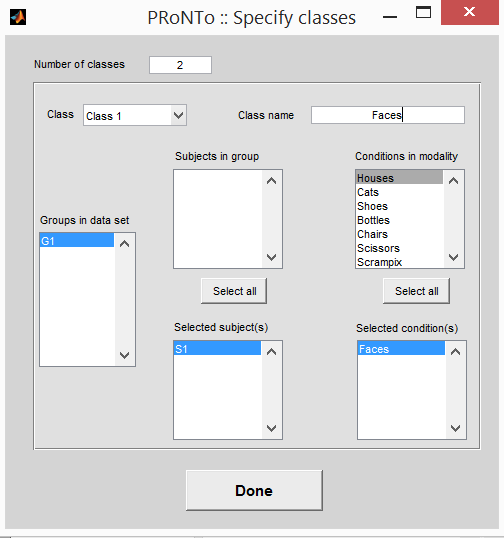
\includegraphics[height=9cm]{images/Tutorial/classification/specifyClasses.png}
	\caption{`Specify classes' GUI.}
	\label{fig:specifyClasses}
\end{figure}
	
	\item Select the `Binary support vector machine' option, in the `Machine' field;
	
	\item Leave the option `Optimize hyper-parameter' tick box unchecked and `Cross-Validation Scheme' (internal loop) as it is; 
	
	\item Select the `Leave One Block Out' cross-validation scheme (external loop);
	
	\item In the `Data operations' box, select the `Sample averaging (within block)' option, which corresponds to a temporal compression of the data within each block, and `Mean centre features using training data' option. Then, the `Specify model' window should look similar to Figure \ref{fig:finalModel};
	
	\begin{figure}[h!]
	\centering
		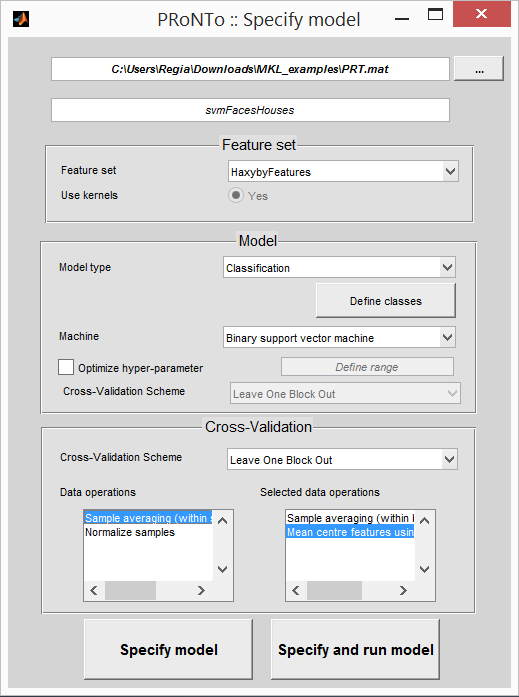
\includegraphics[scale=0.7]{images/Tutorial/classification/finalModel.png}
	\caption{`Specify model' GUI final configuration.}
	\label{fig:finalModel}
\end{figure}
	
	\item Click on `Specify and run model' and the model will be immediately estimated, therefore there is no need to use the `Run model' module in this case;

	\item If you do not wish to average the scans within each block (i.e. to do temporal compression), go back to the `Specify model' window, give another name to the model and select the same options mentioned above, except in the data operations part. Here, choose only the `Mean centre features using training data' option. Finish by clicking on the `Specify and run model' button.
\end{itemize}

%--------------------------------------------------------------------

\subsection{Display model (optional step)}

\begin{itemize}
\item To review the model specification, in the main PRoNTo GUI, click on `Review kernel \& CV' and a new window will open, `Review Model Specification' (Figure \ref{fig:reviewModel});

\begin{figure}[h!]
	\centering
		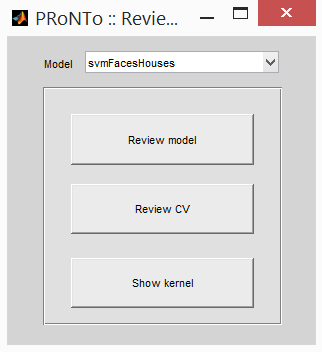
\includegraphics[scale=0.7]{images/Tutorial/classification/reviewModel.png}
	\caption{Review CV \& kernel window.}
	\label{fig:reviewModel}
\end{figure}

\item Select the model, `svmFacesHouses', from the list at the top and click on `Review model'; then, select one class from the list of `Class' to see which groups, subjects and conditions this class comprises (Figure \ref{fig:reviewModelClass});



\begin{figure}[h!]
	\centering
		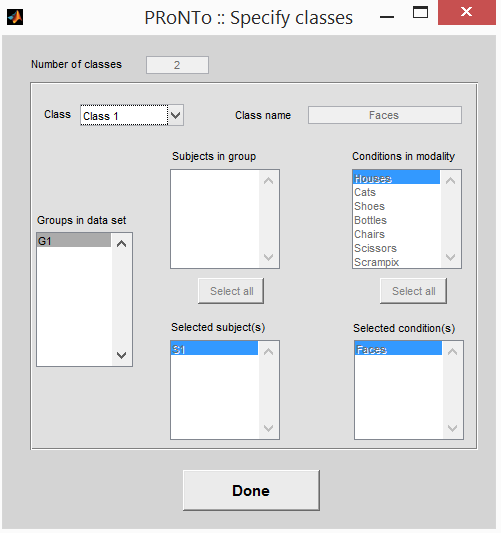
\includegraphics[scale=0.7]{images/Tutorial/classification/reviewModelClass.png}
	\caption{Review model specification window to Class 1.}
	\label{fig:reviewModelClass}
\end{figure}

\item To review the data and cross-validation matrix click on `Review CV' (Figure \ref{fig:reviewCV}). For more information on what these matrices mean, please consult the previous chapters of the manual;

\begin{figure}[h!]
	\centering
		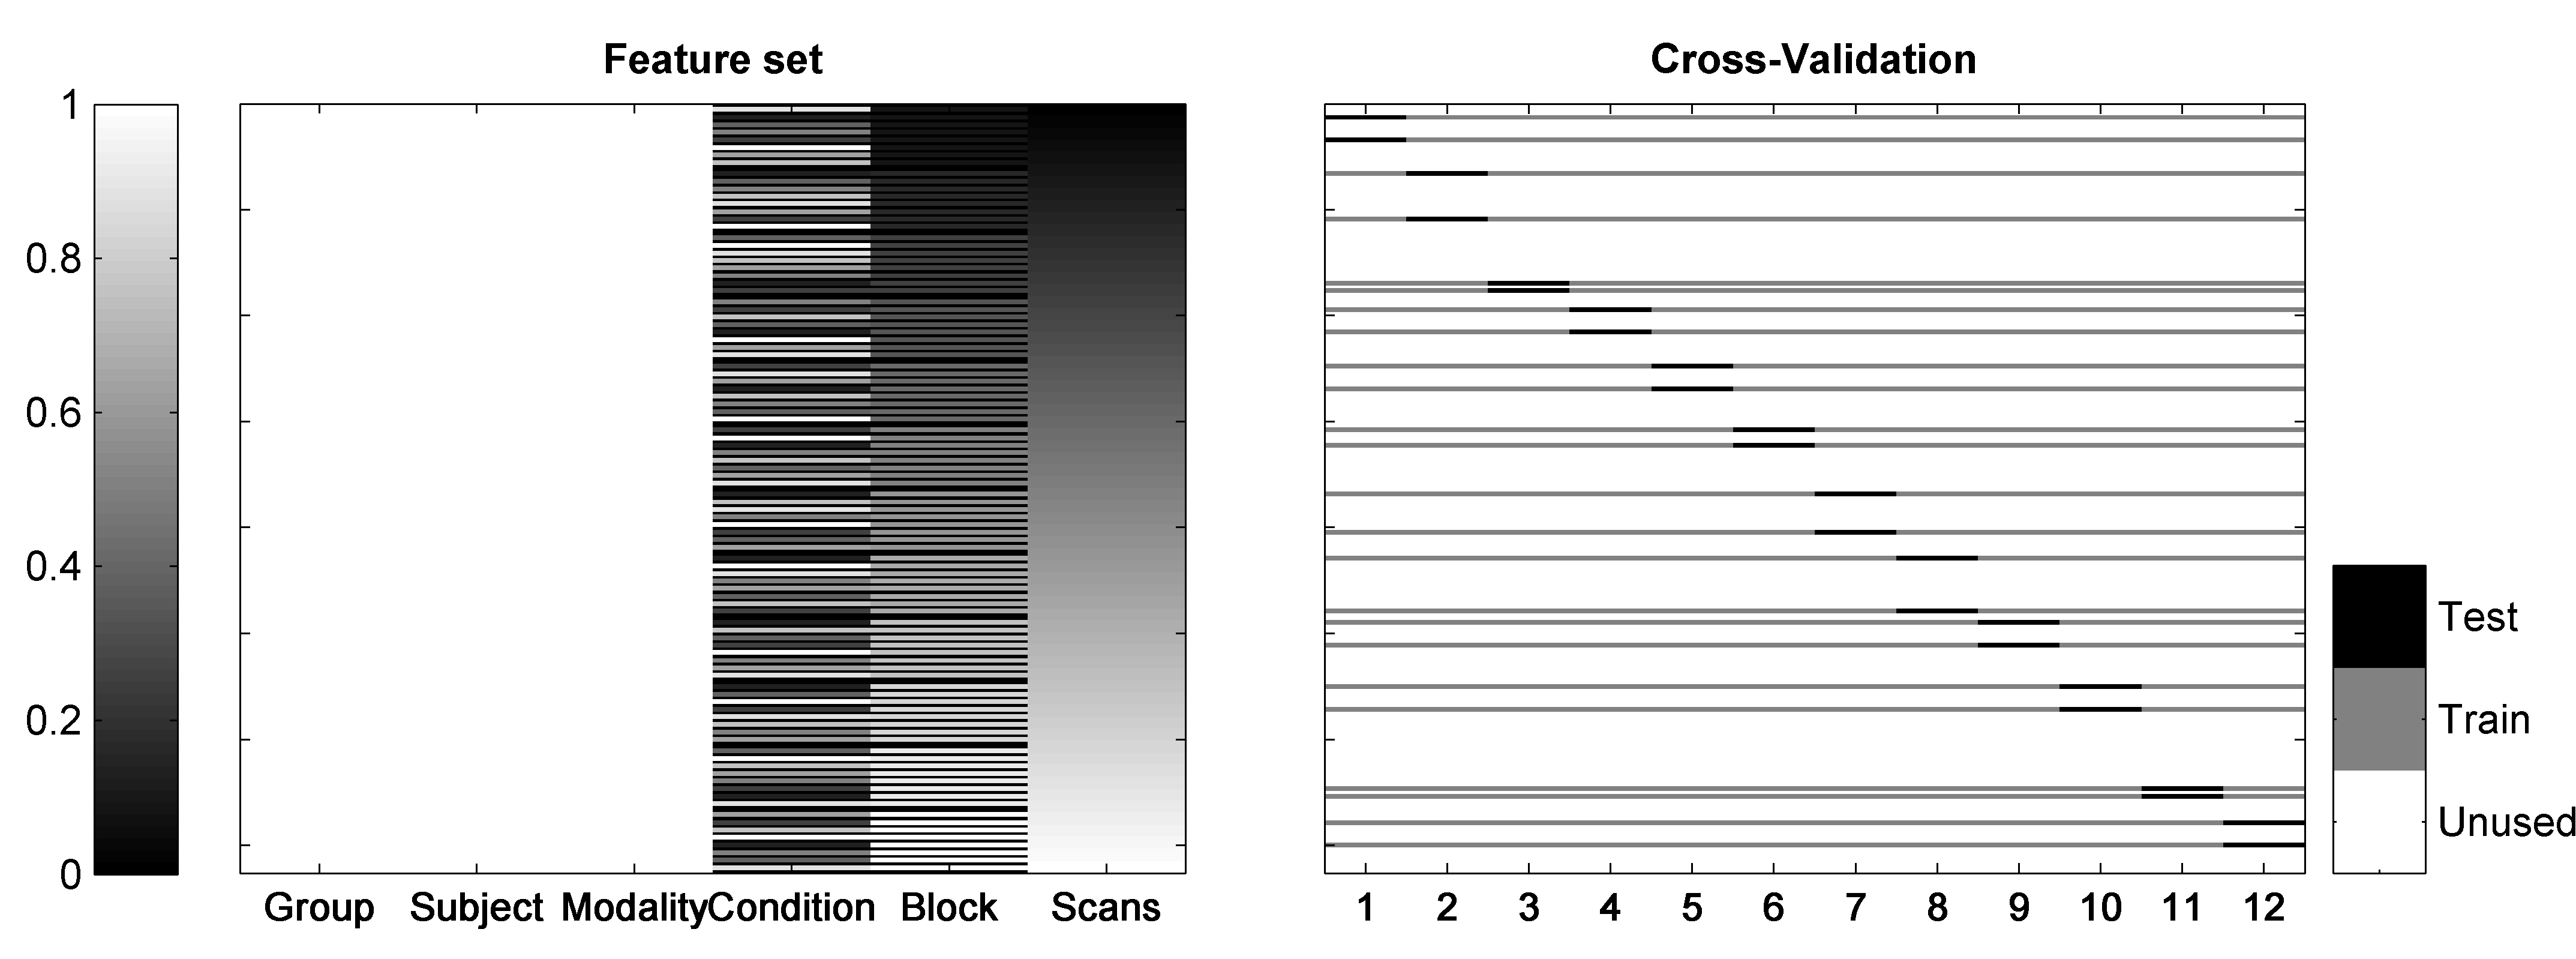
\includegraphics[scale=0.7]{images/Tutorial/classification/reviewCV.png}
	\caption{Data and cross-validation matrix from `Review CV' option.}
	\label{fig:reviewCV}
\end{figure}

\item To review the kernel, click on `Show kernel' (Figure \ref{fig:reviewKernel}).

\begin{figure}[h!]
	\centering
		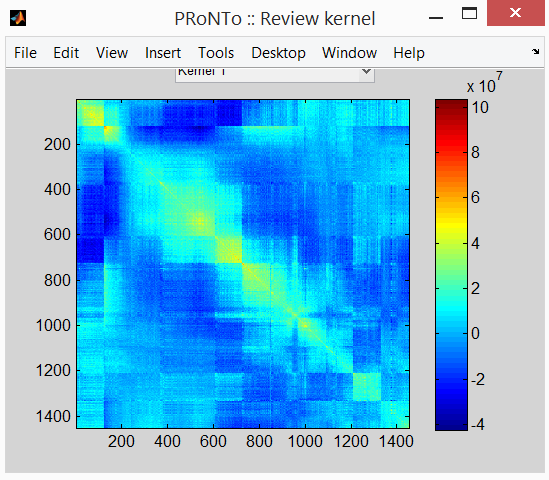
\includegraphics[scale=0.7]{images/Tutorial/classification/reviewKernel.png}
	\caption{Kernel matrix used for classification.}
	\label{fig:reviewKernel}
\end{figure}

\end{itemize}

%----------------------------------------------------

\subsection{Compute weights (optional step)}

\begin{itemize}
\item In PRoNTo's main window, click on `Compute weights' and a new window will open, `Compute weights' (Figure \ref{fig:computeWeights});

\begin{figure}[h!]
	\centering
		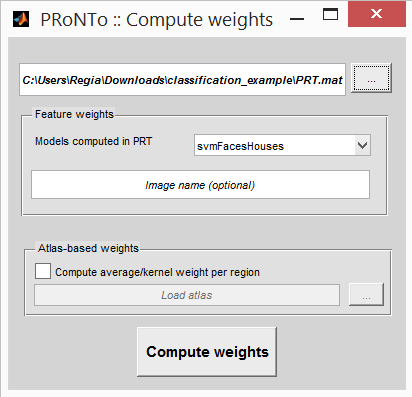
\includegraphics[scale=0.7]{images/Tutorial/classification/computeWeights.png}
	\caption{`Compute weights' GUI.}
	\label{fig:computeWeights}
\end{figure}

\item Select the `PRT.mat' file;

\item Select the model from the list to `Models computed in PRT', `svmFacesHouses' model;

\item Leave the option `Compute average/kernel weight per region' tick box unchecked;

\item Click on `Compute weights' button. Computations will be displayed on the MATLAB command window.

\end{itemize}

%------------------------------------------------------------------

\subsection{Display results}
\label{display_results}

\begin{itemize}
	
	\item In PRoNTo's main window, click on `Display results' and select the `PRT.mat' file. This will open the main results window (Figure \ref{fig:results});
	
\begin{figure}[h!]
	\centering
		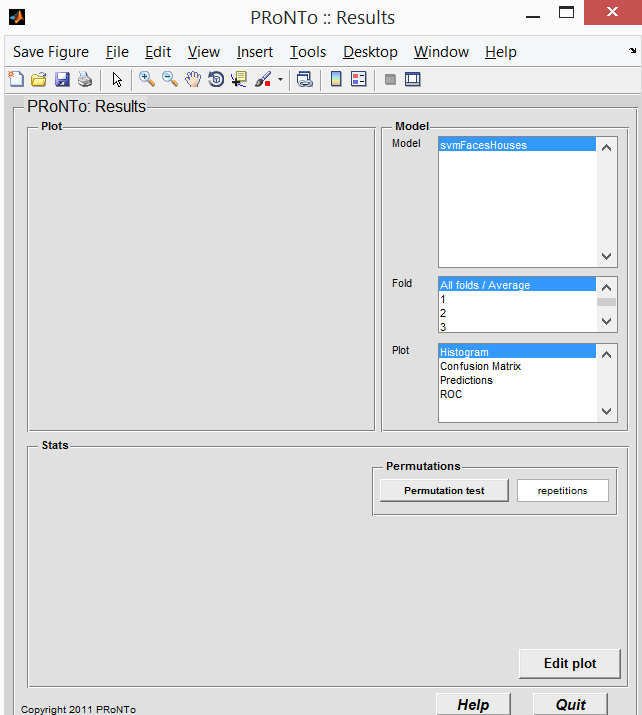
\includegraphics[scale=0.6]{images/Tutorial/classification/results.png}
	\caption{`Results' GUI.}
	\label{fig:results}
\end{figure}
	
	
	\item In the `Model' panel, select the model that you want to view, `svmFacesHouses'. The performance should be similar to the one in Figure \ref{fig:stats};
	
	\begin{figure}[h!]
	\centering
		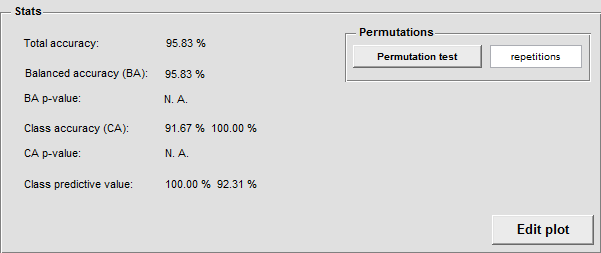
\includegraphics[scale=0.75]{images/Tutorial/classification/stats.png}
	\caption{Summary for model's performance.}
	\label{fig:stats}
\end{figure}
	
	\item In the `Results' window, one can select a different plot in the `Plots' list;
	
	
	\item Finally, to check the significance of the results, run a permutation test by clicking on `Permutation test' button with 100 repetitions. Results will be displayed on the MATLAB prompt (Figure \ref{fig:permutations}). Please note that 100 repetitions is a small amount, if possible, this should be greater (e.g. 1000).

\begin{figure}[h!]
	\centering
		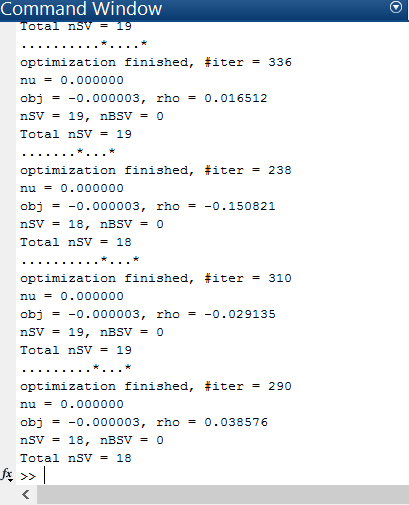
\includegraphics[height=9cm]{images/Tutorial/classification/permutations.png}
	\caption{Sample of the MATLAB window after the permutation test (100 repetitions).}
	\label{fig:permutations}
\end{figure}

\end{itemize}
	
%------------------------------------------------------------------

\subsection{Display weights}

\begin{itemize}
	
	\item In PRoNTo's main window, click on `Display weights' and select the `PRT.mat' file. This will open the `Model interpretation' window (Figure \ref{fig:modelInterpretationMain});
	
	\begin{figure}[h!]
	\centering
		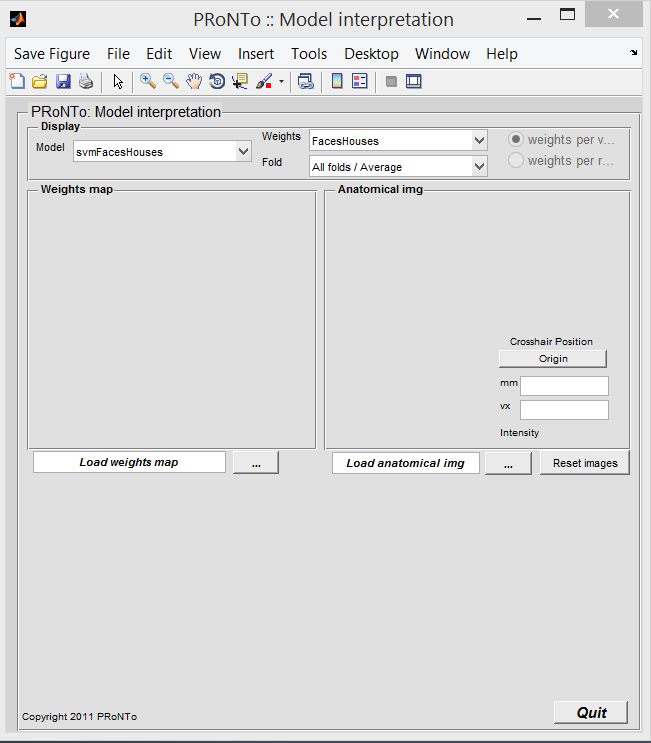
\includegraphics[scale=0.6]{images/Tutorial/classification/modelInterpretationMain.png}
	\caption{`Model interpretation' GUI.}
	\label{fig:modelInterpretationMain}
\end{figure}

	
	\item By clicking on `Model', svmFacesHouses, an image will appear in the `Weights map' box; and to show the `Anatomical img' you have to load an anatomical image for reference. A template image can be found in SPM's canonical folder (`single\_subj\_T1` file). The final window will look similar to the one shown in the Figure \ref{fig:modelInterpretation}.

\begin{figure}[h!]
	\centering
		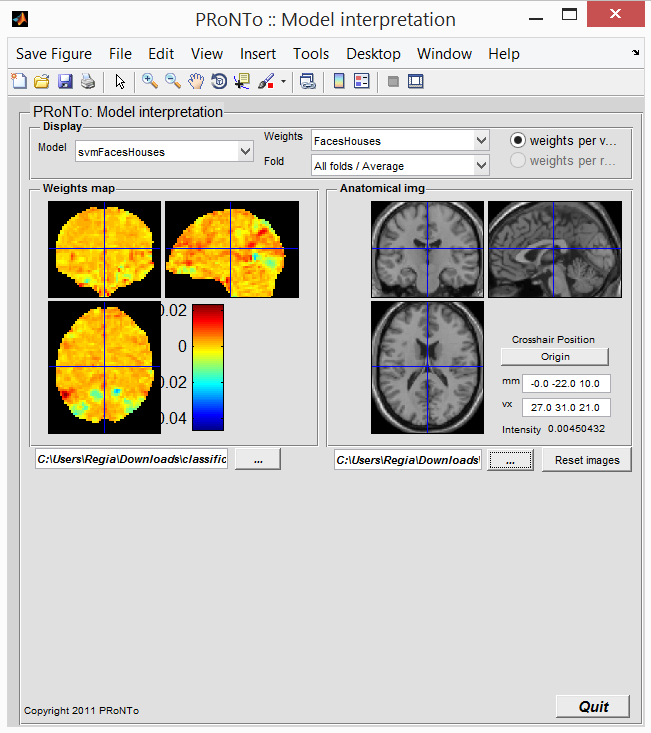
\includegraphics[height=10cm]{images/Tutorial/classification/modelInterpretation.png}
	\caption{`Model interpretation' GUI with results.}
	\label{fig:modelInterpretation}
\end{figure}
	
\end{itemize}

%=====================================================



%=====================================================

\section{Batch analysis}
\label{sec:Batch_analysis_svm}

This tutorial will now show how to analyse the same data but using the {\tt matlabbatch} system.

Once again, create a new directory where you wish to save the results. On the main interface of PRoNTo click on the `Batch' button to open the `{\tt matlabbatch}'. Alternatively, type `prt\_batch' on the MATLAB command window. On the menu bar of the batch, there is a PRoNTo menu with the 5 options shown in the main steps interface (Figure \ref{fig:batch}).

\begin{figure}[h!]
	\centering
		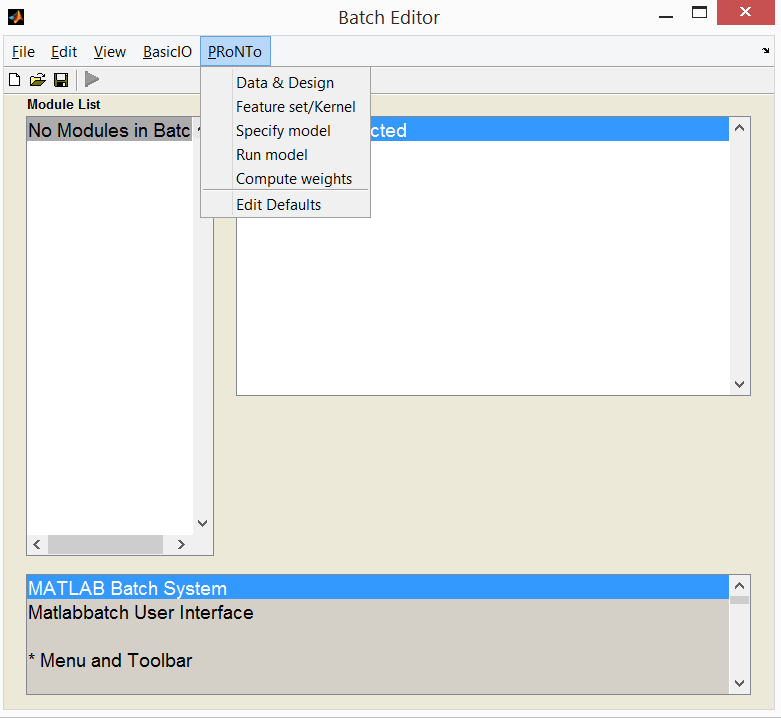
\includegraphics[scale=0.6]{images/Tutorial/classification/batch.png}
	\caption{Menu PRoNTo in the main {\tt matlabbatch} window.}
	\label{fig:batch}
\end{figure}

%--------------------------------------------------------------

\subsection{Data \& Design}

\begin{itemize}

	\item Click on `Data \& Design' in the PRoNTo menu (Figure \ref{fig:batchData});
	
	\begin{figure}[h!]
	
	\centering
		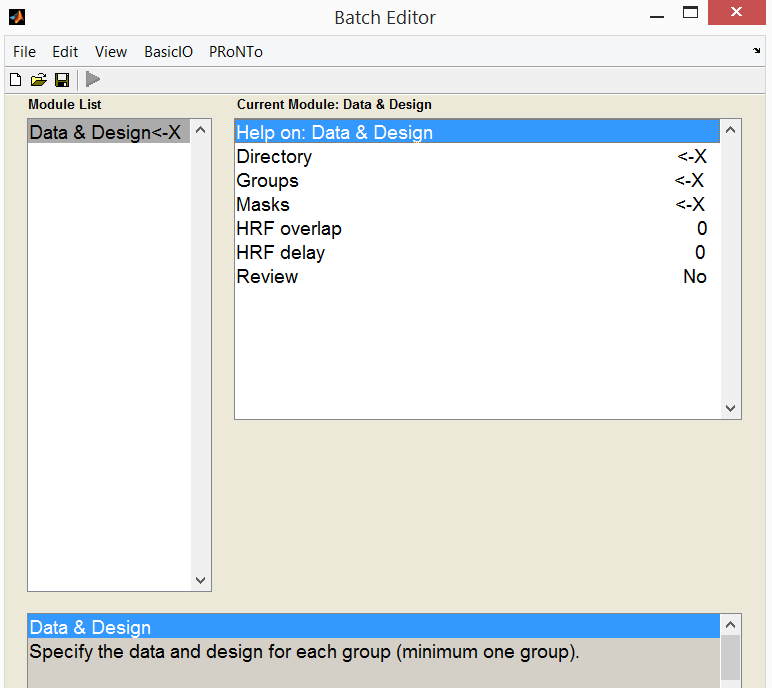
\includegraphics[scale=0.6]{images/Tutorial/classification/batchData.png}
	\caption{Data and design module in {\tt matlabbatch}. }
	\label{fig:batchData}
	
	\end{figure}

	\item In the `Directory' field, select a directory where the `PRT.mat' file will be saved. There are three ways of editing all fields in {\tt matlabbatch}: (i) by using the right mouse button and clicking on the current option, (ii) clicking on current button in the window or (iii) by double clicking;
	
	\item In the `Groups' field:
 	
		\begin{itemize}
		
		\item Add one group;
		
		\item In the field `Name', provide a name without spaces to that group, e.g. `G1'; 
		
		\item In the field `Select by', select the `Subjects' option and add one subject;
		
		\item Add one modality for this subject and provide a name, e.g. `fMRI'; define the interscan interval of 2.5 seconds; and in the field `Scans', select all the image files available in the fMRI directory of the Haxby dataset;	
		
		\item In the `Data \& Design' field, choose `Load SPM.mat' option. This file is available with the Haxby dataset on PRoNTo's website\footnote{http://www.mlnl.cs.ucl.ac.uk/pronto/prtdata.html} inside the folder Haxby\_dataset/design/. The batch editor should look similar to the one in Figure \ref{fig:batchGroups};	
		
		\begin{figure}[h!]
	\centering
		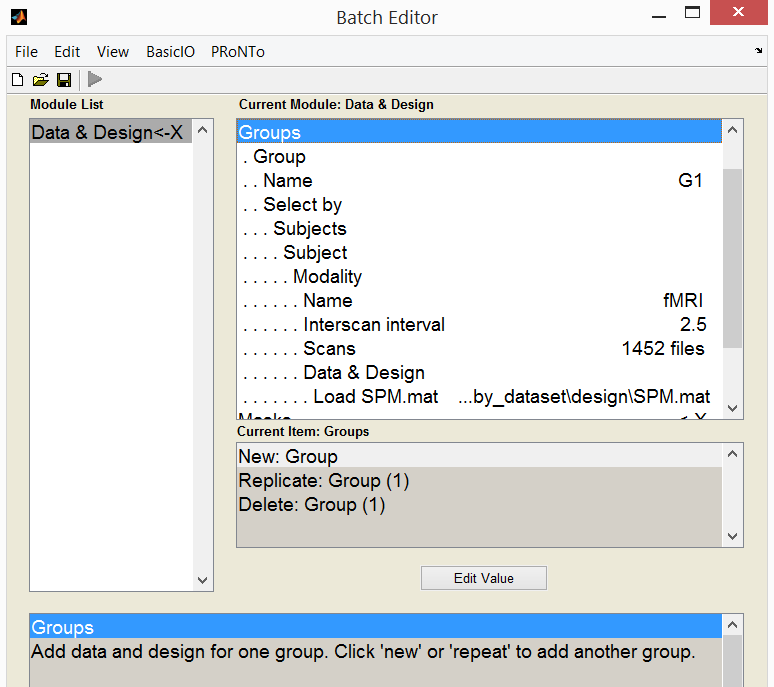
\includegraphics[scale=0.6]{images/Tutorial/classification/batchGroups.png}
	\caption{Data and design module in {\tt matlabbatch}. }
	\label{fig:batchGroups}
	\end{figure}
				
		
		\begin{itemize}
	
			\item In case there is no `SPM.mat' file available to use, create a new	design by selecting the option `Specify design'. Choose how many conditions you have, which in this case are 8 conditions (corresponding to the 8 categories of images). The unit in which the onsets/durations are read is `Scans'. Write the names, onsets and durations of each condition (Figure \ref{fig:batchSpecifyDesign});
	
\begin{figure}[h!]
	\centering
		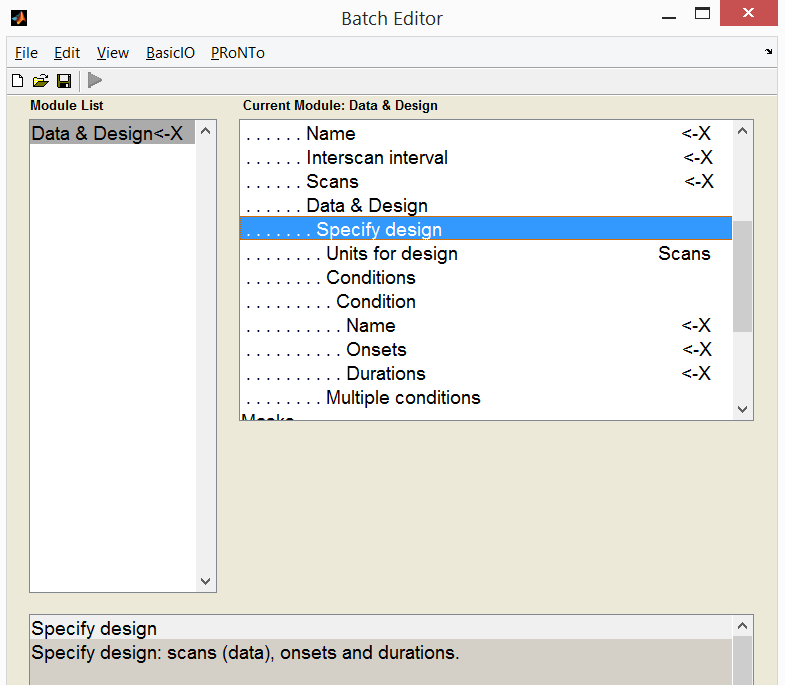
\includegraphics[scale=0.6]{images/Tutorial/classification/batchSpecifyDesign.png}
	\caption{Data and design module. The `Specify design' option.}
	\label{fig:batchSpecifyDesign}
\end{figure}
	
	\end{itemize}

		\end{itemize}
	
	\item In the `Masks' field, add a new modality and provide the same modality name, `fMRI'; and select the `whole\_brain' mask available in the masks directory of the Haxby dataset. The name of the modality here has to be exactly the same as in `Modalities', otherwise it will not work;
	
	%checar aqui
	
	\item Leave the `HRF overlap' and the `HRF delay' fields as default;
	
	\item In the `Review' field, select `Yes' if you would like to review your data and design in a separate window. Otherwise, leave as it is, i.e. `No'.


\end{itemize}

%------------------------------------------------------------

\subsection{Feature set / Kernel}

\begin{itemize}
	\item Click on `Feature set / Kernel' option on PRoNTo's {\tt matlabbatch} menu (Figure \ref{fig:batchFeature});
	
	\begin{figure}[h!]
	\centering
		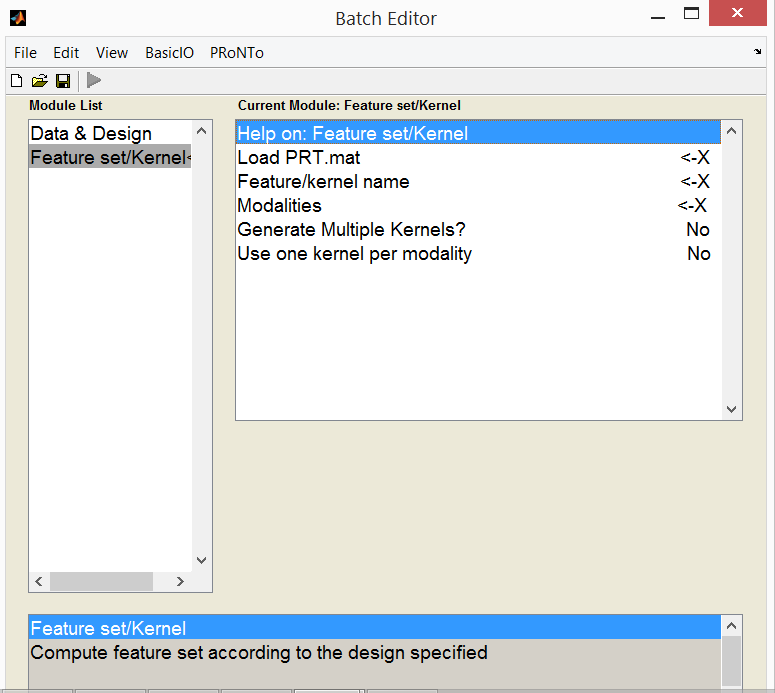
\includegraphics[scale=0.6]{images/Tutorial/classification/batchFeature.png}
	\caption{Feature set/Kernel module in {\tt matlabbatch}. }
	\label{fig:batchFeature}
\end{figure}
	
	\item With `Load PRT.mat' field selected, click on the `Dependency' button to associate the `PRT.mat' file created in the previous `Data \& Design' step (Figure \ref{fig:batchDependency}) or click on the `Select files' button to browse where `PRT.mat' file was saved;
	
	 	
\begin{figure}[h!]
	\centering
		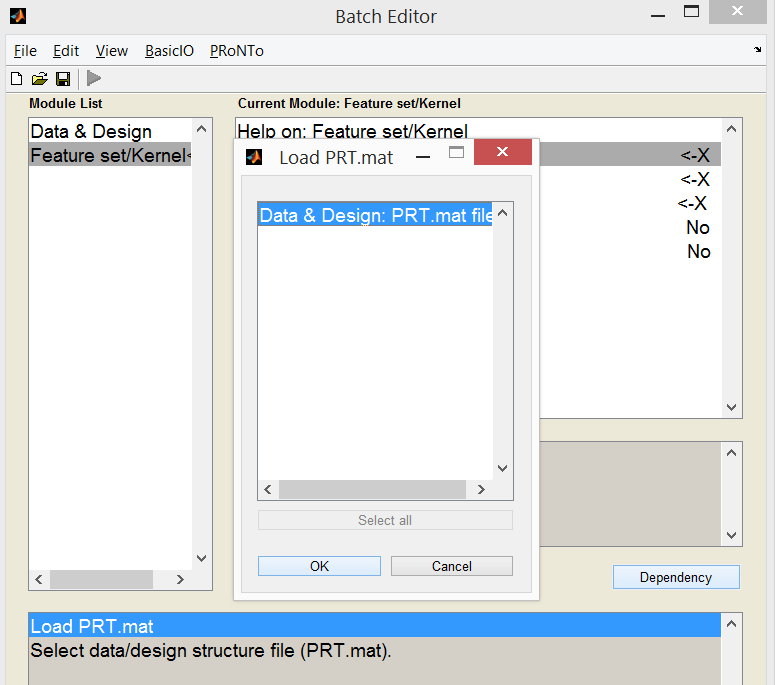
\includegraphics[scale=0.6]{images/Tutorial/classification/batchDependency.png}
	\caption{Feature set / Kernel module in {\tt matlabbatch}. This window is called to establish a dependency connection with the previous `Data and design' module.}
	\label{fig:batchDependency}
\end{figure}
	
	\item Provide a name to the `Feature/kernel' set, e.g. `HaxbyFeatures';
	
	\item Add one modality and select the modality name with the `Dependency' button\footnote{Or type it in manually, `fMRI', but the name needs to be {\it exactly} the same as the one specified in the `Data \& Design' module.}(Data \& Design:Mod\#1 name);
	
		\begin{itemize}
	
	\item In the `Scans/Conditions' field , select the `All scans' option;
	
	\item In the `Voxels to include' field, select `All voxels' option, this means we are not entering an additional second-level mask;
	
			\begin{itemize}
			\item This is an optional step. In the `Voxels to include' options, the user can specify a `second-level' mask, which would define regions of interest (ROIs) on which the classification can be performed. In this case, select the `fusiform\_gyrus' mask;
			\end{itemize}
	
	\item In the `Detrend' field, select `Polynomial detrend' option with order 1;
	
	\item In the `Scale input scans' field, select `No scaling' option;
	
	\item Leave `Load Atlas' as default. After all these steps, the batch editor should look similar to the one in Figure \ref{fig:batchModality};
	
	\begin{figure}[h!]
	\centering
		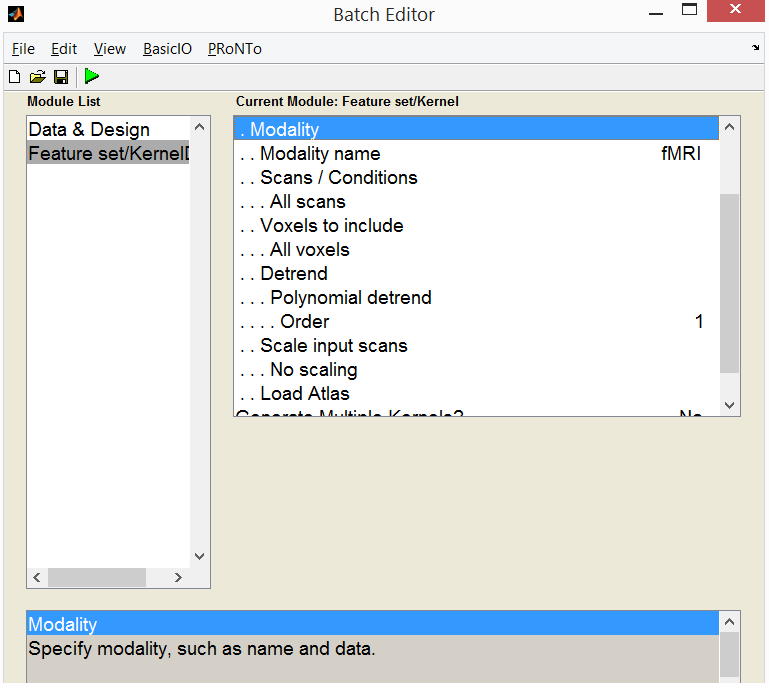
\includegraphics[scale=0.6]{images/Tutorial/classification/batchModality.png}
	\caption{Feature set / Kernel module. Selected parameters in the Modality option.}
	\label{fig:batchModality}
\end{figure}
	
	\end{itemize}
	
	\item Leave the `Generate Multiple Kernels' and the `Use one kernel per modality' fields as default.
	

\end{itemize}

%--------------------------------------------------------

\subsection{Specify model}

\begin{itemize}

\item Click on `Specify model' option on PRoNTo's {\tt matlabbatch} menu (Figure \ref{fig:batchSpecifyModel});
	
	\begin{figure}[h!]
	\centering
		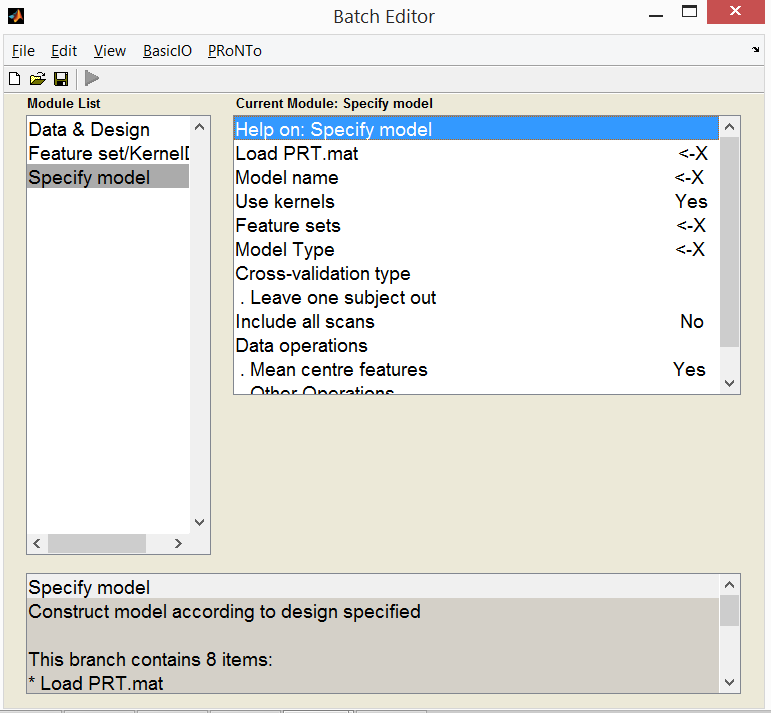
\includegraphics[scale=0.6]{images/Tutorial/classification/batchSpecifyModel.png}
	\caption{Specify model module in {\tt matlabbatch}.}
	\label{fig:batchSpecifyModel}
\end{figure}
	
	\item With `Load PRT.mat' field selected, click on `Dependency' button to associate the `PRT.mat' file created in the previous `Feature set / Kernel' step (Figure \ref{fig:batchDependency2}) or click on `Select files' button to browse where `PRT.mat' file was saved;
	
\begin{figure}[h!]
	\centering
		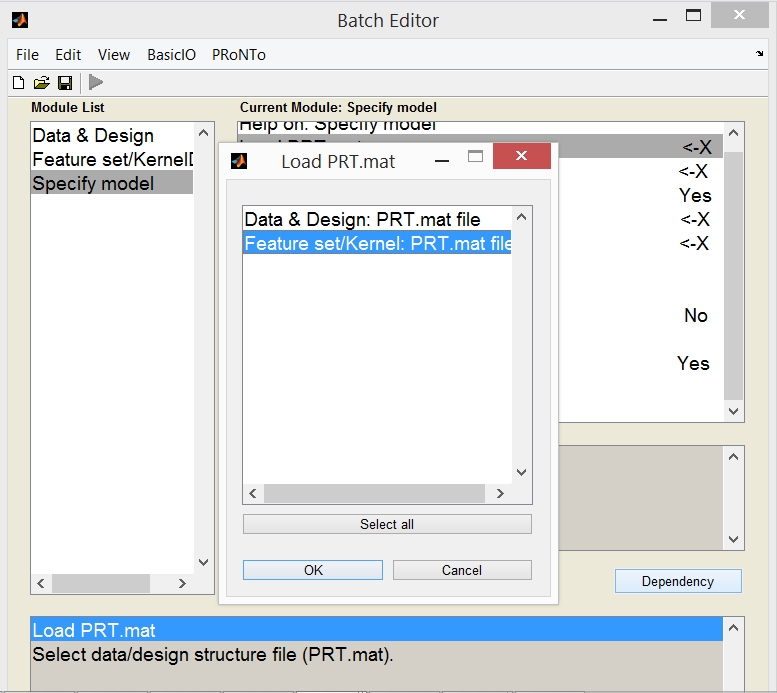
\includegraphics[scale=0.6]{images/Tutorial/classification/batchDependency2.png}
	\caption{Specify model module in {\tt matlabbatch}. This window is called to establish a dependency connection with the previous `Feature set / Kernel' module.}
	\label{fig:batchDependency2}
\end{figure}

	\item Provide a name to the model, e.g. `svmFacesHouses'; 
	
	\item Leave the `Use kernels' field as it is, i.e. `Yes';
	
	\item In the `Feature sets' field, select the feature set name with the `Dependency' button\footnote{or write it {\it exactly} as previously defined in the `Feature set / Kernel' module (option `Feature set/Kernel: Feature/kernel name'), here `HaxbyFeatures'.};
	
	\item Select the `Classification' model type:
	
		\begin{itemize}
		
		\item Add 2 new classes;
		
		\item For Class (1) write `Faces' on the name field and add one group. Select the group name from the `Data \& Design' module (`Data \& Design:Group\#1 name') with the `Dependency' button\footnote{Or write it {\it exactly}, as previously defined in the Data \& Design' module, here `G1'}. Similarly, for Class (2) write `Houses' on the name field and add the group created in the `Data \& Design' module, `G1';	
		
		\item In the `Subjects' field, type `1' (only subject 1 is selected);
		
		\item In the `Conditions / Scans' field, select the `Specify Conditions' option and add a new condition. Provide a name for this condition, i.e. for Class (1) `Faces' and for Class (2) `Houses'. Note that this name needs to be spelled exactly as specified in the `Data \& Design' module: if you simply loaded an `SPM.mat' file for the design, you {\it must} know the names of the conditions;
		
		\item After all this steps, the batch editor should look similar to the one in Figure \ref{fig:batchClass}	
	
	\begin{figure}[h!]
	\centering
		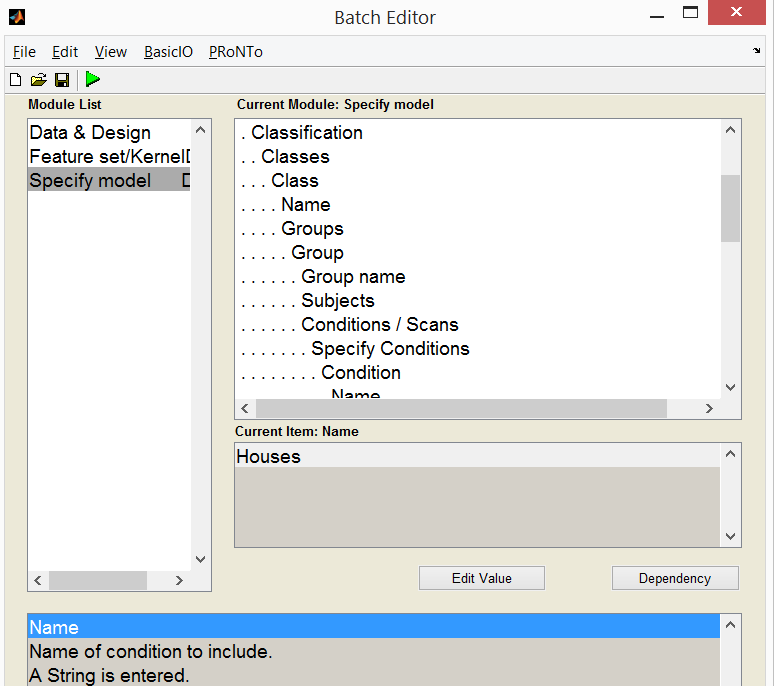
\includegraphics[scale=0.6]{images/Tutorial/classification/batchClass.png}
	\caption{Specify model module. Selected parameters in the Class option.}
	\label{fig:batchClass}
\end{figure}

		\end{itemize}			
		
	\item In the `Machine' field:
	
	\begin{itemize}
	\item Select the `SVM Classification' option;	
	
	\item Leave the `Optimize hyper-parameter' field as it is, i.e. `No';
	
	\item Leave the `Soft-margin hyper-parameter' field as it is, i.e. `1';
	
	\item Leave the `Cross validation type for hyper-parameter optimization' field as it is, i.e. `Leave one subject out';  
	
	
	\end{itemize}
	
	\item In the `Cross-validation type' field, select `Leave one block out' option;
	
	\item Leave the `Include all scans' field as it is, i.e. `No';

	\item In the `Data operations' field:
	
		\begin{itemize}
		\item  Leave the `Mean centre features' field as it is, i.e. `Yes'; 
				
		\item  Leave the `Other Operations' field as it is, i.e. `No operations';
		\end{itemize}
	
\end{itemize}

%----------------------------------------------------------

\subsection{Run model}

\begin{itemize}

	\item Click on the `Run model' option on PRoNTo's {\tt matlabbatch} menu (Figure \ref{fig:batchRun});
	
	\begin{figure}[h!]
	\centering
		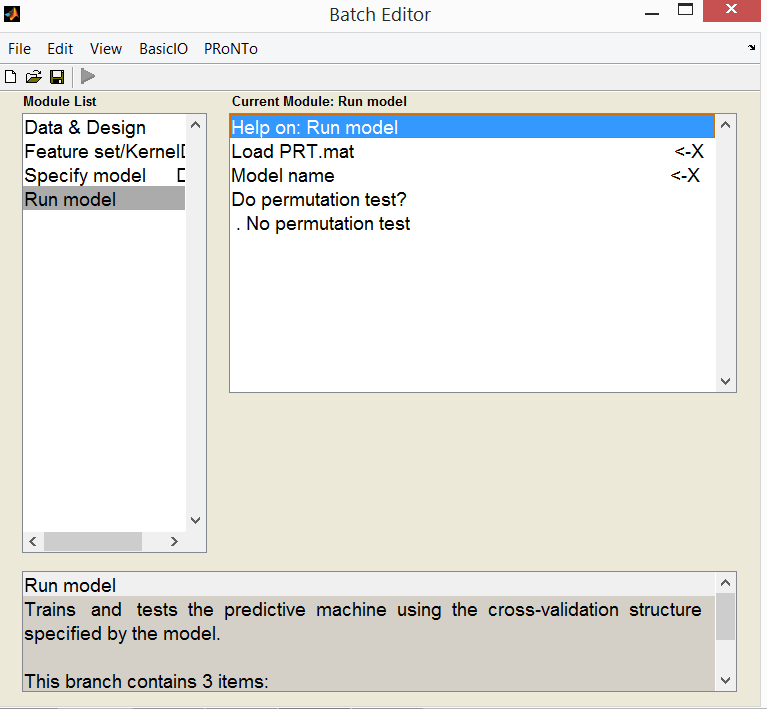
\includegraphics[scale=0.6]{images/Tutorial/classification/batchRun.png}
	\caption{Run model module in {\tt matlabbatch}.}
	\label{fig:batchRun}
\end{figure}
	
	
	\item  With the `Load PRT.mat' field selected, click on the `Dependency' button to associate the `PRT.mat' file created in the previous `Specify model' step;
	
	\item Select the model name from the `Specify model' module with the `Dependency' button\footnote{Or write it {\it exactly}, as previously defined in the `Specify model' module, here `svmFacesHouses'};

	\item In the field `Do permutation test?', select `yes' with 100 repetitions or leave as default (1000 repetitions).

\end{itemize}
%-----------------------------------------------------

\subsection{Compute weights (optional step)}

\begin{itemize}

	\item Click on the `Compute weights' option on PRoNTo's {\tt matlabbatch} menu (Figure \ref{fig:batchWeights});
	
	\begin{figure}[h!]
	\centering
		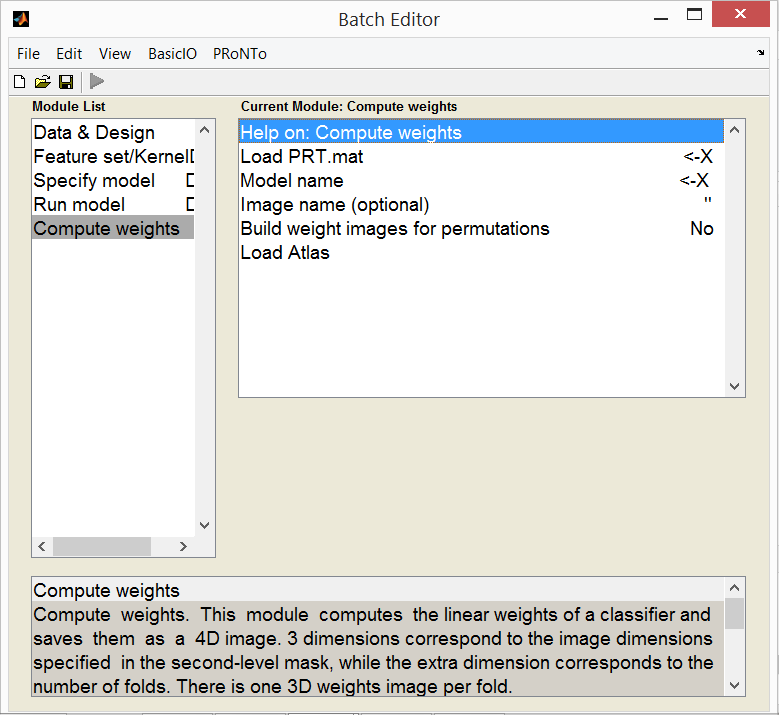
\includegraphics[scale=0.6]{images/Tutorial/classification/batchWeights.png}
	\caption{Compute weights module in {\tt matlabbatch}.}
	\label{fig:batchWeights}
\end{figure}

	\item With `Load PRT.mat' field selected, click on the `Dependency' button to associate the `PRT.mat' file created in the previous `Run model' step;
	
	\item Select the model name from the `Specify model' module with the `Dependency' button;
	
	\item It's optional to define a name for the image; 
	
	\item Leave the `Build weights images for permutations' field as it is, i.e. `No'; 
	
	\item Leave the `Load Atlas' field as default.

\end{itemize}

Finally, save the batch (e.g. as batch\_run\_all.m) and click on the `Run Batch' option, in the `File menu'. The batch file created can then be opened and edited for further analyses. The results will be the same as those obtained using the GUI (see Section \ref{display_results}  of this chapter). Please note that in this case the `Sample averaging (within block)' operation was not selected when specifying the model. In order to obtain the same results as before, the model has to use the same data operations.
